\chapter{Fundamentação teórica}
%%%%%%%%%%%%%%%%%%%%%%%%%%%%%%%%%%%%%%%%%%%%%%%%%%%%%%%%%%%%%%%%%%%%%%
Neste capitulo, apresentamos uma síntese da revisão bibliográfica realizada para embasar a metodologia adotada no desenvolvimento e simulação do ADPLL. São abordados os conceitos básicos de um sintetizador de frequência, o protocolo de comunicação \textit{Bluetooth} e a importância dos circuitos e dispositivos CMOS. Esses tópicos são fundamentais para compreender o funcionamento do ADPLL e sua aplicação em sistemas de comunicação sem fio. A revisão bibliográfica oferece uma base sólida para o desenvolvimento do projeto, fornecendo os conhecimentos necessários para explorar as características, desempenho e aplicações do ADPLL.

%%%%%%%%%%%%%%%%%%%%%%%%%%%%%%%%%%%%%%%%%%%%%%%%%%%%%%%%%%%%%%%%%%%%%%
\section{Sintetizador de frequência}
%%%%%%%%%%%%%%%%%%%%%%%%%%%%%%%%%%%%%%%%%%%%%%%%%%%%%%%%%%%%%%%%%%%%%%
Em sistemas de comunicação sem fio a presença de um circuito sintetizador de frequência é essencial. O circuito sintetizador de frequência é responsável por gerar a frequência central de um canal em um sistema de comunicação de Rádio Frequência (RF). Cada canal possui uma faixa de frequência especifica de operação, desta forma o circuito do Sintetizador deve ser capaz de permitir ajustes de frequência pequenos.

O circuito Sintetizador de frequência gera as frequências necessária como um múltiplo de uma referência do Oscilador de Cristal Controlado por Temperatura (TXCO, do inglês \textit{Temperature-Controlled Crystal Oscillator}). O TXCO papel fundamental na performance do sintetizador, é responsavél por fornece uma frequência estável e precisa e com baixo valor de ruido de fase. De acordo com \cite{lascari2000accurate} negligenciar seus efeitos em um sintetizador pode acarretar em resultados inesperados após a concepção do circuito.

O processo de síntese de frequência ocorre através de técnicas de geração e mistura de sinais. Primeiramente, a referência de TXCO fornece uma frequência estável e precisa. Em seguida, o sintetizador de frequência utiliza circuitos internos, como divisores de frequência e circuitos de fase, para manipular e multiplicar a frequência da referência, produzindo assim a frequência desejada.


%%%%%%%%%%%%%%%%%%%%%%%%%%%%%%%%%%%%%%%%%%%%%%%%%%%%%%%%%%%%%%%%%%%%%%
\subsection{PLL}
%%%%%%%%%%%%%%%%%%%%%%%%%%%%%%%%%%%%%%%%%%%%%%%%%%%%%%%%%%%%%%%%%%%%%%
PLL (\textit{Phase-Locked-Lopp}) é um circuito Sintetizador de frequência comumente utilizado. PLL é composto por diversos blocos, alguns deles são: osciladores controlados por tensão VCO (\textit{Voltage-Controlled Oscillator}), divisores programáveis, comparadores de fase DFF (Detectores de Fase e Frequência), bombas de carga CP ((\textit{Charge Pump}) e Filtros Passa Baixas LPF ((\textit{Low Pass Filters}). 

Os blocos que compõem um PLL são apresentados na Figura \ref{fig:pll_blocks}.
A utilização de uma realimentação negativa no circuito permite um controle tanto de frequência como de fase para a saída.

\begin{figure}[h!]
	\caption{Blocos de um PLL.}
	\begin{center}
		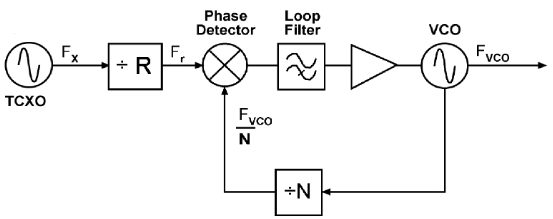
\includegraphics[scale=0.6]{img/pll_blocos.png}
	\end{center}
	\fonte{\citeonline{barrett_1999_fractionalintegern}}
	\label{fig:pll_blocks}
\end{figure}

O PLL utiliza o VCO como elemento central. O sinal de saída do VCO, dividido por um fator N, é comparado com a frequência de referência do TXCO, dividida por R, pelo  \textit{Phase-Detector}. Após a comparação, o sinal resultante passa pelo\textit{Loop filter}, responsável por eliminar ruídos e interferências. A saída do \textit{Loop filter} é uma tensão que controla a tensão aplicada ao VCO, permitindo ajustar e manter a frequência de saída em sincronia com a frequência de referência \cite{barrett_1999_fractionalintegern}.

%%%%%%%%%%%%%%%%%%%%%%%%%%%%%%%%%%%%%%%%%%%%%%%%%%%%%%%%%%%%%%%%%%%%%%
\subsubsection{Integer-N PLL}
%%%%%%%%%%%%%%%%%%%%%%%%%%%%%%%%%%%%%%%%%%%%%%%%%%%%%%%%%%%%%%%%%%%%%%

PLLs convencionais também conhecidos como \textit{Integer-N PLL} são capazes de gerar apenas frequências de valores N vezes a frequência do TXCO, onde N é um valor inteiro, desta forma a resolução de frequência é definida pela frequência de referência utilizada. 

A frequência de saída é definida como:

\begin{equation}
	F_{VCO} = N \cdot F_{ref}
	\label{eq:fvco_integer_PLL}
\end{equation}



%%%%%%%%%%%%%%%%%%%%%%%%%%%%%%%%%%%%%%%%%%%%%%%%%%%%%%%%%%%%%%%%%%%%%%
\subsubsection{Fractional-N PLL }
%%%%%%%%%%%%%%%%%%%%%%%%%%%%%%%%%%%%%%%%%%%%%%%%%%%%%%%%%%%%%%%%%%%%%%
Em um \textit{fractional-N} PLL a frequência de saída pode ser ajustada como uma fração da frequência de referência. Esse ajuste fracional é necessário em sistemas de comunicação para o ajuste correto da frequência central de canal utilizado. 

\textit{Fractional-N} PLL utiliza uma topologia similar ao do \textit{Integer-N} PLL, com adição de um acumulador, uma maquina de altera que o divisor entre (N e N+1) durante um estado bloqueado. Esta variação faz com que a média torne-se um valor fracional entre N e N+1, proporcionando um ajuste de frequência também fracional. 

A frequência de saída é definida como:

\begin{equation}
	F_{VCO} = (N + F) \cdot F_{ref}
	\label{eq:fvco_fractional_PLL}
\end{equation}
Onde, $F$ é um valor entre $0$ e $1$. 

%%%%%%%%%%%%%%%%%%%%%%%%%%%%%%%%%%%%%%%%%%%%%%%%%%%%%%%%%%%%%%%%%%%%%%
\section{ADPLL}
%%%%%%%%%%%%%%%%%%%%%%%%%%%%%%%%%%%%%%%%%%%%%%%%%%%%%%%%%%%%%%%%%%%%%%


%%%%%%%%%%%%%%%%%%%%%%%%%%%%%%%%%%%%%%%%%%%%%%%%%%%%%%%%%%%%%%%%%%%%%%
%\textit{Energy Harvesting} 
%%%%%%%%%%%%%%%%%%%%%%%%%%%%%%%%%%%%%%%%%%%%%%%%%%%%%%%%%%%%%%%%%%%%%%


%%%%%%%%%%%%%%%%%%%%%%%%%%%%%%%%%%%%%%%%%%%%%%%%%%%%%%%%%%%%%%%%%%%%%%
\subsection{DCO}
%%%%%%%%%%%%%%%%%%%%%%%%%%%%%%%%%%%%%%%%%%%%%%%%%%%%%%%%%%%%%%%%%%%%%%

%%%%%%%%%%%%%%%%%%%%%%%%%%%%%%%%%%%%%%%%%%%%%%%%%%%%%%%%%%%%%%%%%%%%%%
\subsection{Loop Filter}
%%%%%%%%%%%%%%%%%%%%%%%%%%%%%%%%%%%%%%%%%%%%%%%%%%%%%%%%%%%%%%%%%%%%%%

%%%%%%%%%%%%%%%%%%%%%%%%%%%%%%%%%%%%%%%%%%%%%%%%%%%%%%%%%%%%%%%%%%%%%%
\subsection{TDC}
%%%%%%%%%%%%%%%%%%%%%%%%%%%%%%%%%%%%%%%%%%%%%%%%%%%%%%%%%%%%%%%%%%%%%%


%%%%%%%%%%%%%%%%%%%%%%%%%%%%%%%%%%%%%%%%%%%%%%%%%%%%%%%%%%%%%%%%%%%%%%
\section{Trabalhos correlatos}
%%%%%%%%%%%%%%%%%%%%%%%%%%%%%%%%%%%%%%%%%%%%%%%%%%%%%%%%%%%%%%%%%%%%%%


%%%%%%%%%%%%%%%%%%%%%%%%%%%%%%%%%%%%%%%%%%%%%%%%%%%%%%%%%%%%%%%%%%%%%%

